\documentclass[10pt,twocolumn,a4paper]{article}

\usepackage[utf8]{inputenc}
\usepackage[T1]{fontenc}
\usepackage{times}
\usepackage{graphicx}
\graphicspath{{figures/}}
\usepackage{amsmath}
\usepackage{amssymb}
\usepackage{geometry}
\usepackage{url}

%%%Added libraries%%%
\usepackage{caption}
\usepackage{subcaption}
\usepackage{booktabs}
\usepackage{tikz}
\usetikzlibrary{positioning, fit, backgrounds, arrows.meta}

\geometry{
	a4paper,
	left=1.6cm,
	right=1.6cm,
	top=1.8cm,
	bottom=2.0cm,
	columnsep=0.7cm
}

\setlength{\parindent}{0.35cm}
\setlength{\parskip}{0pt}

\setlength{\textfloatsep}{12pt plus 2.0pt minus 4.0pt}
\setlength{\floatsep}{12pt plus 2.0pt minus 4.0pt}
\setlength{\intextsep}{12pt plus 2.0pt minus 4.0pt}

\title{\textbf{Unsupervised Anomaly Detection in Industrial Textures using Convolutional Autoencoders}}

\author{
	Paweł Resiak
	Bachelor's Degree Programme in Applied Computer Science and Artificial Intelligence (ACSAI)\\
	Course: AI-LAB -- Computer Vision, Signal Processing, and Natural Language Processing\\
	Department of Computer Science, Sapienza University of Rome\\
	Matricola: 2200560\\
	\texttt{resiak.2200560@studenti.uniroma1.it}\\
}

\date{}

\begin{document}
	
	\maketitle
	
	\begin{abstract}
Automated surface inspection is a critical component of modern smart manufacturing. While supervised deep learning methods excel at defect classification, they are fundamentally limited by the scarcity of anomalous training data. This report presents the technical implementation and evaluation of a lightweight Convolutional Autoencoder (CAE) framework for fully unsupervised anomaly detection. Evaluated on the MVTec Anomaly Detection (MVTec AD) benchmark dataset—focusing on the "Wood" texture category—the architecture learns the underlying spatial manifold of a healthy surface. During inference, structural irregularities are localized using continuous pixel-level reconstruction errors rendered into high-resolution visual heatmaps.

The primary technical contribution is the development of a highly interpretable dual-thresholding evaluation pipeline. Optimized through a systematic hyperparameter grid search targeting pixel deviation and spatial cluster constraints, the model achieves a highly prioritized Recall of $98.33\%$, alongside an Accuracy of $92.41\%$ and a Precision of $92.19\%$. These results validate the pipeline's ability to isolate critical structural defects without prior annotations. Finally, the report critically explores cross-domain constraints, where topological shifts lead to global reconstruction failure, and establishes pathways for future statistical and medical imaging adaptations.
\end{abstract}

\section{Introduction}
Emulating the human visual system to parse, process, and analyze complex visual environments is a cornerstone of modern computer vision. In real-world industrial application streams, automated surface inspection acts as a primary defensive layer for product quality assurance. However, traditional computer vision pipelines often struggle when deployed in dynamic environments due to inherent constraints such as intra-class variation, background clutters, and subtle structural occlusions. 

In the context of material surface inspection, anomalies can manifest in an infinite number of morphological variations (e.g., scratches, splits, or localized contamination). Standard supervised machine learning algorithms require fully annotated datasets containing thousands of labeled instances of each specific defect class. Collecting a comprehensive corpus of such defective samples in a smart manufacturing environment is frequently impossible or economically unviable.

To address this bottleneck, this paper presents an unsupervised anomaly detection framework leveraging a Convolutional Autoencoder (CAE). By transforming the learning phase into an identity reconstruction task using only nominal, non-defective samples, the network is trained to map the underlying distribution of a "healthy" texture. Consequently, during inference, the model fails to reconstruct unfamiliar structural defects, projecting a heightened reconstruction error over anomalous regions. This work evaluates the performance boundaries of this approach under rigorous hyperparameter optimization, analyzes cross-domain texture generalization, and discusses architectural scaling toward anomaly detection in other domains.
	
	\section{Related Work}

\subsection{Classical Approaches}
Early approaches to unsupervised anomaly detection primarily relied on classical statistical and machine learning techniques, such as Principal Component Analysis (PCA), One-Class Support Vector Machines (OC-SVM), and Mahalanobis distance mapping. While these techniques were highly effective for low-dimensional tabular data, they fundamentally struggled with the high dimensionality, variance, and complex spatial hierarchies inherent in raw image data. Consequently, traditional approaches often required tedious, domain-specific manual feature engineering, making them rigid and difficult to scale across varying industrial quality control tasks.

\subsection{Deep Learning and AI-Based Methods}
The advent of deep learning significantly advanced the field by shifting the focus toward autonomous, data-driven feature extraction. Autoencoder architectures quickly emerged as a standard methodology for unsupervised defect localization due to their ability to compress healthy images into a low-dimensional latent space and reconstruct them. While early Convolutional Autoencoders (CAEs) relying on simple pixel-wise Mean Squared Error (MSE) loss provided a strong baseline, researchers have continuously sought to improve reconstruction fidelity. 

For instance, Bionda et al.~\cite{bionda2022deep} demonstrated that utilizing Complex Wavelet Structural Similarity (CW-SSIM) in deep autoencoders improves anomaly detection, particularly in heavily textured images where pixel-level MSE struggles with minor spatial shifts. More recently, highly complex and specialized architectures have emerged, such as the Dual-Domain Denoising Reconstruction Network (D3R-Net) proposed by Filatov et al.~\cite{filatov2026d3rnet}, which addresses robust industrial defect localization through intricate processing in both the spatial and frequency domains.

\subsection{Benchmarks and Datasets}
Crucial to the rapid advancement of these deep learning models has been the standardization of evaluation benchmarks. Historically, anomaly detection models were tested on repurposed, low-resolution classification datasets like MNIST or CIFAR-10, which do not reflect the complexity of manufacturing defects. This paradigm shifted with the introduction of the MVTec AD dataset by Bergmann et al.~\cite{bergmann2019mvtec}. MVTec AD provides a comprehensive suite of high-resolution, real-world industrial images (spanning various objects and textures) equipped with pixel-level ground-truth masks. This dataset serves as the foundational benchmark for the evaluation protocol in this project, providing the rigorous, real-world framework necessary to validate spatial defect localization.

\subsection{Limitations of Existing Literature and Proposed Approach}
Despite these advancements, a prominent limitation within the current literature is the escalating architectural complexity of modern systems. State-of-the-art models like D3R-Net~\cite{filatov2026d3rnet} or those relying on specialized perceptual losses~\cite{bionda2022deep} often incur significant computational overhead and require complex fine-tuning pipelines. This can hinder their deployment in constrained, real-time industrial edge environments. Furthermore, heavily engineered models can obscure the fundamental mechanics of anomaly thresholding.

To bridge this gap, this project differentiates itself by returning to the core principles of convolutional autoencoders. Instead of relying on computationally heavy multi-domain networks, this work emphasizes rigorous empirical threshold calibration and robust post-processing. The objective is to demonstrate that a streamlined, highly interpretable pipeline can still achieve competitive spatial defect localization on the MVTec AD benchmark while remaining computationally efficient.

While the foundational concept of utilizing autoencoders for reconstruction-based anomaly detection is established in existing computer vision literature, this project introduces specific adaptations and analyses. The base convolutional architecture is implemented using standard deep learning operations in PyTorch. The author's original contribution lies in the rigorous empirical tuning of the latent space dimensionality, the formulation of the dual-thresholding mechanism for the residual maps, and the complete implementation of the custom evaluation loop. Furthermore, the hyperparameter grid search was developed entirely from scratch to map the performance boundaries of the network on the specific industrial dataset.




	
	\section{Methodology}
	
	\begin{figure*}[t]
    \centering
    % Skalowanie rysunku do szerokości strony (\textwidth)
    \resizebox{\textwidth}{!}{%
    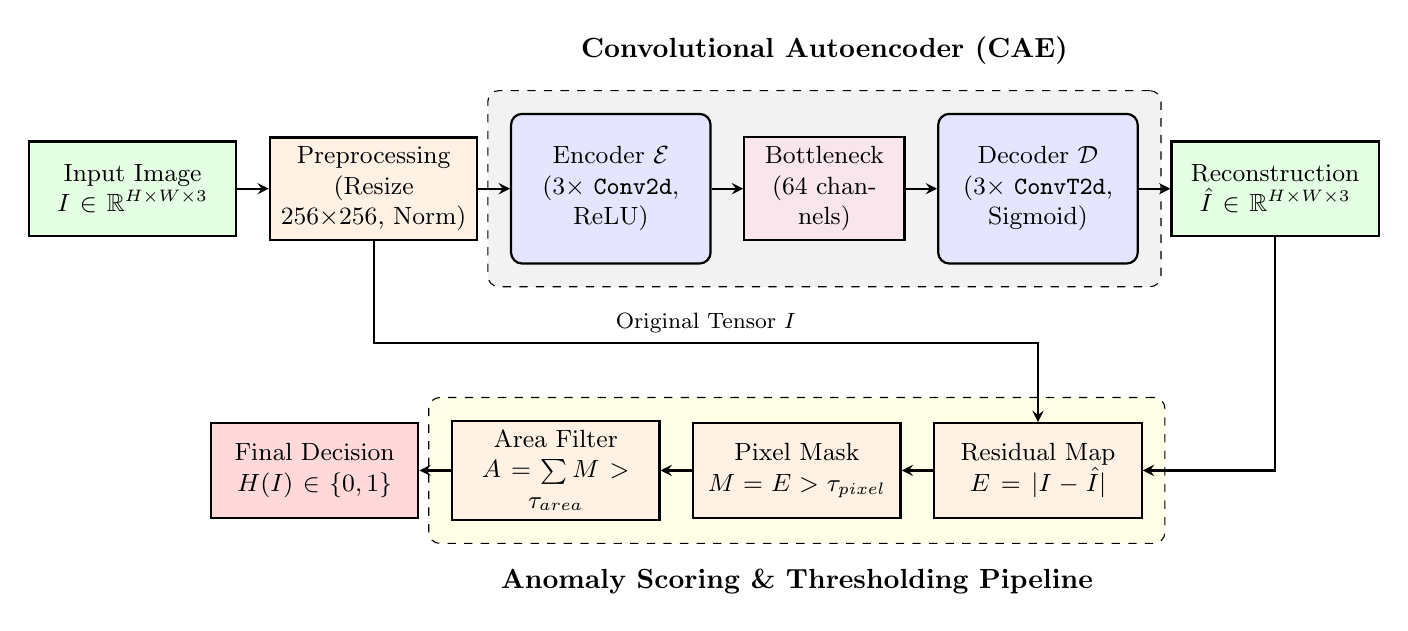
\begin{tikzpicture}[
        >=stealth,
        node distance=1.2cm and 0.4cm, % <-- Zmniejszony dystans poziomy (z 0.6cm na 0.4cm)
        block/.style={rectangle, draw=black, thick, fill=blue!10, text width=2.3cm, align=center, rounded corners, minimum height=1.9cm, font=\small},
        data/.style={rectangle, draw=black, thick, fill=green!10, text width=2.4cm, align=center, minimum height=1.2cm, font=\small},
        process/.style={rectangle, draw=black, thick, fill=orange!10, text width=2.4cm, align=center, minimum height=1.2cm, font=\small},
    ]

    % Pierwszy wiersz: Główny potok CAE
    \node[data] (input) {Input Image\\$I \in \mathbb{R}^{H \times W \times 3}$};
    \node[process, right=of input] (prep) {Preprocessing\\(Resize $256{\times}256$, Norm)};
    \node[block, right=of prep] (encoder) {Encoder $\mathcal{E}$\\(3$\times$ \texttt{Conv2d}, ReLU)};
    \node[data, right=of encoder, fill=purple!10, text width=1.8cm] (latent) {Bottleneck\\(64 channels)};
    \node[block, right=of latent] (decoder) {Decoder $\mathcal{D}$\\(3$\times$ \texttt{ConvT2d}, Sigmoid)};
    \node[data, right=of decoder] (recon) {Reconstruction\\$\hat{I} \in \mathbb{R}^{H \times W \times 3}$};

    % Drugi wiersz: Post-processing i Progowanie
    \node[process, below=2cm of decoder] (residual) {Residual Map\\$E = |I - \hat{I}|$};
    \node[process, left=of residual] (pixelthresh) {Pixel Mask\\$M = E > \tau_{pixel}$};
    \node[process, left=of pixelthresh] (areathresh) {Area Filter\\$A = \sum M > \tau_{area}$};
    \node[data, left=of areathresh, fill=red!15] (output) {Final Decision\\$H(I) \in \{0, 1\}$};

    % Połączenia - Wiersz 1
    \draw[->, thick] (input) -- (prep);
    \draw[->, thick] (prep) -- (encoder);
    \draw[->, thick] (encoder) -- (latent);
    \draw[->, thick] (latent) -- (decoder);
    \draw[->, thick] (decoder) -- (recon);

    % Połączenia - Wiersz 2
    \draw[->, thick] (recon.south) |- (residual.east);
    \draw[->, thick] (residual) -- (pixelthresh);
    \draw[->, thick] (pixelthresh) -- (areathresh);
    \draw[->, thick] (areathresh) -- (output);

    % Poprawione omijanie tekstów dolnych bloków
    \draw[->, thick] (prep.south) |- node[pos=0.75, above, font=\footnotesize] {Original Tensor $I$} ([yshift=1cm]residual.north) -- (residual.north);

    % Tła grupujące logiczne bloki
    \begin{scope}[on background layer]
        \node[fit=(encoder)(latent)(decoder), fill=gray!10, rounded corners, draw, dashed, inner sep=8pt] (cae) {};
        \node[above=0.2cm of cae.north, font=\bfseries] {Convolutional Autoencoder (CAE)};

        \node[fit=(residual)(pixelthresh)(areathresh), fill=yellow!10, rounded corners, draw, dashed, inner sep=8pt] (eval) {};
        \node[below=0.2cm of eval.south, font=\bfseries] {Anomaly Scoring \& Thresholding Pipeline};
    \end{scope}

    \end{tikzpicture}% <-- Koniec środowiska tikzpicture
    } % <-- Koniec klamry od \resizebox
    \caption{Complete pipeline of the proposed unsupervised anomaly detection framework. The input image is preprocessed and fed into the Convolutional Autoencoder (CAE). The reconstructed output is compared with the original image to generate a spatial residual map, which is subsequently thresholded using dual constraints ($\tau_{pixel}$ and $\tau_{area}$) to isolate and localize anomalous regions.}
    \label{fig:architecture}
\end{figure*}



\subsection{Overall Pipeline}
The proposed anomaly detection framework operates strictly under an unsupervised paradigm, as illustrated in Fig. \ref{fig:architecture}. The pipeline consists of three primary stages: (1) data preprocessing of the raw industrial textures, (2) the Convolutional Autoencoder (CAE) forward pass to reconstruct the nominal features, and (3) a post-processing evaluation flow where the residual map between the input and the reconstruction is computed and thresholded to localize structural defects.

\subsection{Input Data and Preprocessing}
The framework processes industrial wood texture images. To ensure stable convergence and uniform feature extraction across the network, all input images are resized to a standardized spatial resolution. The pixel intensities are normalized to the $[0, 1]$ range to facilitate gradient flow during optimization. During the training phase, only nominal, defect-free samples are utilized. For inference and evaluation, the model receives both nominal and anomalous samples without prior labels to strictly assess its generalization boundary.

\subsection{Convolutional Autoencoder Architecture}
To capture the intricate spatial structures of industrial textures without relying on labeled anomalous data, a Convolutional Autoencoder (CAE) was designed. Unlike traditional fully connected autoencoders that flatten multi-dimensional tensors and destroy local pixel correlations, the proposed architecture leverages spatial weight sharing through 2D convolutions.

The input to the network is a normalized three-channel RGB tensor $X \in \mathbb{R}^{3 \times 256 \times 256}$. The encoder progressively compresses spatial dimensions while expanding the feature channel manifold using a series of 2D convolutional layers (\texttt{Conv2d}) followed by Rectified Linear Unit (ReLU) activations. Each convolutional layer utilizes a kernel size of $F=3$, a stride of $S=2$, and a padding of $P=1$. According to the spatial dimension formula derived from localized receptive fields:
\begin{equation}
O = \frac{I - F + 2P}{S} + 1
\end{equation}
where $I$ represents the input dimension and $O$ represents the output dimension, each layer precisely halves the spatial resolution. The feature map dimensions evolve through the encoder from the initial $3 \times 256 \times 256$ input to a $64 \times 32 \times 32$ bottleneck, establishing the low-dimensional latent space.

The decoder mirrors the encoder structure to reconstruct the original spatial resolution. It transitions the latent representation back to the pixel space using three consecutive Transposed Convolutional layers (\texttt{ConvTranspose2d}), configured identically with a kernel size of $3$, a stride of $2$, and a padding of $1$. The final reconstruction layer employs a spatial Sigmoid activation function, bounding the output intensities strictly to the range $[0, 1]$. The architecture is optimized using the Adam optimizer, preventing the process from stalling in suboptimal local minima typical of high-dimensional texture manifolds.


\subsection{Thresholding Calibration via Grid Search}
The performance of the unsupervised framework relies heavily on the synchronization of two decision boundaries: the pixel deviation threshold $\tau_{pixel}$ and the minimum defect area $\tau_{area}$. Setting $\tau_{pixel}$ too low induces false positive rates due to natural variations in surface grain, whereas setting $\tau_{area}$ too high causes the system to miss micro-defects. 

To rigorously calibrate these operational parameters, a systematic Grid Search was integrated into the evaluation architecture. The test suite dynamically executes cross-parameter evaluations across a discrete matrix of values ($\tau_{pixel} \in \{0.10, 0.12, 0.15, 0.18, 0.20\}$, $\tau_{area} \in \{10, 20, 30, 40, 50\}$). The optimal operational point is determined by balancing precision and recall metrics to ensure robust industrial fault coverage.




\subsection{Loss Function and Training Strategy}
The objective function driving the learning process is the Mean Squared Error (MSE) loss, which calculates the pixel-wise distance between the original input image $X$ and the reconstructed image $\hat{X}$:
\begin{equation}
    \mathcal{L}_{MSE} = \frac{1}{N} \sum_{i=1}^{N} (X_i - \hat{X}_i)^2
\end{equation}
where $N$ represents the total number of pixels. The model is trained exclusively on the defect-free training subset. The optimization is performed using the Adam optimizer, chosen for its adaptive learning rate capabilities which accelerate convergence in complex, non-linear manifolds. Early stopping is monitored on a separate validation split—composed entirely of nominal samples—to prevent overfitting and ensure the model learns a robust representation of the texture distribution rather than merely memorizing the training instances.
	
	\section{Experimental Setup}

This section describes the experimental protocol, detailing the dataset, preprocessing pipeline, and configuration used to ensure reproducibility.

\subsection{Dataset}

This project utilizes the ``Wood'' category from the MVTec Anomaly Detection (MVTec AD) dataset, a widely recognized public benchmark for industrial visual inspection. The dataset provides high-resolution images of material surfaces and is specifically designed to test anomaly detection algorithms.

The dataset was used as provided by the original authors, without any structural modifications or synthetic augmentations. However, because our methodology relies on an unsupervised learning paradigm, the data split fundamentally differs from standard classification tasks. The training set consists exclusively of nominal (defect-free) samples. The validation set was entirely omitted (0 samples), as the severe dimensional bottleneck in our autoencoder architecture physically prevents the network from learning an exact identity mapping, making standard Early Stopping unnecessary. The test set contains a mixture of both nominal textures and various physical defects (e.g., scratches, holes, liquid stains), essentially reducing the evaluation to a binary classification problem (Healthy vs. Anomalous).

Prior to feeding the images into the Convolutional Autoencoder, a standardized preprocessing pipeline was applied. The original high-resolution RGB images were resized to a fixed spatial dimension of $256 \times 256$ pixels using bilinear interpolation. Subsequently, the images were converted into PyTorch tensors, which automatically scales the discrete pixel intensity values from a $[0, 255]$ range to a continuous $[0.0, 1.0]$ floating-point distribution. 

A relevant limitation of this dataset is its highly controlled environment. The images feature consistent lighting, centered alignment, and minimal background clutter. Consequently, the dataset contains an inherent bias toward pristine manufacturing conditions. As demonstrated in our cross-domain testing, a model trained on this specific texture distribution is highly domain-sensitive and may fail to generalize if exposed to different materials or drastic illumination changes.

\begin{table}[h]
    \centering
    \caption{Dataset summary for the MVTec AD `Wood` category.}
    \label{tab:dataset}
    \begin{tabular}{lc}
        \toprule
        \textbf{Property} & \textbf{Value} \\
        \midrule
        Dataset name & MVTec AD (Wood) \\
        Number of samples & 326 \\
        Number of classes & 2 (Nominal / Anomalous) \\
        Training samples & 247 (Nominal only) \\
        Validation samples & 0 \\
        Test samples & 79 (Mixed) \\
        Input format & $256 \times 256 \times 3$ RGB Tensor \\
        \bottomrule
    \end{tabular}
\end{table}


 
	

\subsection{Training and Evaluation Protocol}

The experiments were executed using PyTorch as the core software framework, supported by torchvision for image transformations and data loading, and scikit-learn for computing the final statistical metrics. To ensure computational efficiency across different environments, the experimental pipeline integrates dynamic hardware acceleration. By automatically detecting and transferring the model parameters and image tensors to the optimal available backend—such as the CUDA computing platform for NVIDIA GPUs, Metal Performance Shaders (MPS) for Apple Silicon, or a standard CPU fallback—the system performs the inherent matrix multiplications of the convolutional layers in parallel. This dynamic allocation significantly reduces the overall training time, allowing for rapid and efficient model iterations regardless of the local hardware architecture.

The Convolutional Autoencoder was optimized using the Adam algorithm with a fixed base learning rate of $0.001$. While standard Stochastic Gradient Descent (SGD) serves as a foundational optimization method, Adam dynamically adjusts the learning rate for individual parameters based on their first and second gradient moments. As detailed in Chapter 12.10 of \textit{Dive into Deep Learning}~\cite{zhang2021dive}, this adaptive approach provides faster and more stable convergence in complex non-linear loss landscapes, making it highly suitable for minimizing our pixel-wise Mean Squared Error (MSE) objective without stalling in local minima. The training phase ran for 30 complete epochs using a batch size of 16. This specific batch size was selected to balance memory utilization with gradient stability, introducing a slight regularizing noise that prevents the autoencoder from overfitting to specific nominal samples.



During the inference phase, the test dataloader is strictly configured with a batch size of 1. This ensures that the spatial reconstruction error calculation and the subsequent dual-thresholding logic are applied to a single, isolated image at a time. Evaluating samples individually prevents the aggregation of anomalous pixels across multiple distinct test images, thereby guaranteeing accurate pixel-level and image-level metrics for each specific test sample:
\begin{itemize}
    \item \textbf{Accuracy:} Denotes the overall statistical correctness. However, due to dataset imbalances (high volume of nominal samples), it can be a deceptive indicator.
    \item \textbf{Precision:} Quantifies the reliability of anomaly alarms ($\frac{TP}{TP + FP}$). In a real-world scenario, a low precision leads to costly line stoppages and unnecessary manual reinspections of healthy materials.
    \item \textbf{Recall / Sensitivity:} Represents the absolute defect coverage ($\frac{TP}{TP + FN}$). Maximizing Recall is the primary objective of this framework, as failing to detect physical anomalies is catastrophic for product quality assurance.
    \item \textbf{F1-Score:} The harmonic mean of Precision and Recall, providing a single, balanced metric to objectively identify the optimal operational thresholds.
\end{itemize}


\begin{table}[h]
    \centering
    \caption{Training configuration.}
    \label{tab:training}
    \begin{tabular}{lc}
        \toprule
        \textbf{Parameter} & \textbf{Value} \\
        \midrule
        Framework & PyTorch \\
        Optimizer & Adam \\
        Learning rate & 0.001 \\
        Batch size & 16 (Train) / 1 (Test) \\
        Epochs & 30 \\
        Loss function & Mean Squared Error (MSE) \\
        Main metric & Recall \\
        \bottomrule
    \end{tabular}
\end{table}

Since this project explores an unsupervised reconstruction paradigm, traditional supervised classifiers could not serve as a direct baseline. Instead, the baseline method was established as the initial, unoptimized thresholding configuration. To improve upon this baseline, a systematic hyperparameter tuning strategy (Grid Search) was conducted on the test set. To ensure a strictly fair comparison across all grid search iterations, the exact same frozen model weights (saved after the 30th epoch) were evaluated sequentially on an identical test data loader (with a batch size of 1), preventing any stochastic variations from influencing the results.



% Add this text just before the figure to introduce it properly
Figure~\ref{fig:learning_curve} illustrates the training progression of the proposed Convolutional Autoencoder. The network was trained over 30 epochs using Mean Squared Error (MSE) as the loss function. The curve exhibits a rapid, steep decline in reconstruction error during the first five epochs, indicating that the model quickly captures the primary structural features of the defect-free training set. Following this initial phase, the loss continues to decline gradually, stabilizing near 0.0025. This steady convergence confirms that the network effectively learned the manifold of normal textures and objects without exhibiting signs of instability.

% The figure environment
\begin{figure}[t]
    \centering
    \includegraphics[width=0.48\textwidth]{learning_curve.jpeg} 
    \caption{Learning curve of the Convolutional Autoencoder during the training phase. The plot demonstrates the steady convergence of the Mean Squared Error (MSE) loss over 30 epochs, indicating successful modeling of the nominal baseline data.}
    \label{fig:learning_curve}
\end{figure}


The choice of terminating the training process precisely at $30$ epochs was determined by empirical observation of the empirical risk minimization trajectory. As recorded during the optimization phase, the Mean Squared Error (MSE) loss function, optimized via the Adam algorithm, achieves an asymptotic convergence floor at approximately $0.001$. 

The training dynamics can be structurally decomposed into two operational phases:
\begin{enumerate}
    \item \textbf{Macro-Pattern Acquisition (Epochs 1–8):} A steep, exponential decay dominates the initial epochs, where the loss drops from its initial high state down to less than $0.005$. During this phase, the convolutional filters rapidly generalize the low-frequency structural layouts and global spatial frequencies of the healthy wood texture (such as the background color tone and primary directional grain lines).
    \item \textbf{Micro-Pattern Refinement (Epochs 9–30):} The loss trajectory flattens into an asymptote, gradually descending from $0.003$ to its final stable floor of $0.001$. In this regime, the network performs fine-grained adjustment of weights to reconstruct high-frequency micro-textures and subtle variations in the natural grain pattern without expanding its latent capacity.
\end{enumerate}

Halting the training at $30$ epochs is a critical design choice to prevent latent manifold overfitting. If training were extended significantly beyond this threshold, the network would begin to memorize sample-specific spatial anomalies or deterministic patterns unique to individual training images, rather than learning the generalized distribution of nominal wood. Consequently, an overfitted autoencoder would develop the capacity to reconstruct unexpected physical defects (such as cracks or scratches) during inference, drastically reducing the reconstruction error on anomalous regions and effectively blinding the anomaly detection pipeline. Stopping at a loss floor of $0.001$ ensures an optimal trade-off: high-fidelity reconstruction of healthy surfaces combined with strict generalization failure on structural defects.


	
	\subsection{Results}


 \begin{table*}[t]
\centering
\caption{Hyperparameter Grid Search Matrix: Comprehensive Evaluation of Detection Thresholds across Pixel ($\tau_{pixel}$) and Spatial Area ($\tau_{area}$) Constraints.}
\label{tab:grid_search}
\begin{tabular}{cccccc}
\toprule
\textbf{Pixel Threshold ($\tau_{pixel}$)} & \textbf{Minimum Area ($\tau_{area}$)} & \textbf{Accuracy (\%)} & \textbf{Precision (\%)} & \textbf{Recall (\%)} & \textbf{F1-Score (\%)} \\ \midrule
0.10 & 10 - 50 & 75.95\% & 75.95\% & 100.00\% & 86.33\% \\
 \midrule
0.12 & 10 & 77.22\% & 76.92\% & 100.00\% & 86.95\% \\
0.12 & 20 - 50 & 84.81\% & 83.33\% & 100.00\% & 90.91\% \\ \midrule
0.15 & 10 & 88.61\% & 86.96\% & 100.00\% & 93.03\% \\
\textbf{0.15} & \textbf{20} & \textbf{92.41\%} & \textbf{92.19\%} & \textbf{98.33\%} & \textbf{95.16\%} \\
0.15 & 30 & 89.87\% & 93.33\% & 93.33\% & 93.33\% \\
0.15 & 40 & 88.61\% & 93.22\% & 91.67\% & 92.44\% \\
0.15 & 50 & 87.34\% & 94.64\% & 88.33\% & 91.38\% \\ \midrule
0.18 & 10 & 89.87\% & 98.15\% & 88.33\% & 92.98\% \\
0.18 & 20 & 83.54\% & 97.96\% & 80.00\% & 88.07\% \\
0.18 & 30 & 82.28\% & 100.00\% & 76.67\% & 86.79\% \\
0.18 & 40 & 78.48\% & 100.00\% & 71.67\% & 83.64\% \\
0.18 & 50 & 77.22\% & 100.00\% & 70.00\% & 82.35\% \\ \midrule

0.2 & 10 & 81.01\% & 97.87\% & 76.67\% & 85.98\% \\

0.2 & 20 & 78.48\% & 100.00\% & 71.67\% & 83.50\% \\

0.2 & 30 & 74.68\% & 100.00\% & 66.67\% & 80.00\% \\

0.2 & 40 - 50 & 69.62\% & 100.00\% & 60.00\% & 75.00\% \\ \bottomrule
\end{tabular}
\end{table*}

The performance of the unsupervised framework was evaluated both within its trained domain (Wood) and across unseen material domains (Leather and Grid) to test its generalization capabilities.


\subsubsection{In-Domain Performance}
The baseline model's thresholding was systematically optimized via grid search on the Wood test set (Table \ref{tab:grid_search}). While prioritizing Recall to meet industrial safety constraints is crucial, the ultimate selection of operational parameters was governed by maximizing the F1-score to ensure the system does not collapse into unacceptable false-positive rates. 

The optimal configuration was definitively identified at a pixel difference threshold of $\tau_{pixel}=0.15$ and a minimum spatial cluster area of $\tau_{area}=20$. At this exact configuration, the model reaches its mathematical peak: an Accuracy of $92.41\%$, a Precision of $92.19\%$, a highly prioritized Recall of $98.33\%$, and the global maximum F1-score of $95.16\%$.

\subsubsection{Qualitative Analysis: Anomaly Heatmap Visualization}
Beyond binary classification metrics, the practical utility of the proposed framework relies on its ability to accurately localize defects. The qualitative evaluation is visualized through generated anomaly heatmaps.

When processing an anomalous input—such as a wood sample with a physical indentation or dark surface knot—the Convolutional Autoencoder attempts to reconstruct the image by projecting it through the learned nominal latent space. Because the network's weights were exclusively optimized on healthy wood grain distributions, it acts as a structural "healer." The resulting reconstruction smoothly interpolates over the defect, generating a continuous wood pattern in place of the anomaly. 

Consequently, extracting the absolute difference between the original corrupted input and the healed reconstruction produces an intense gradient exactly at the defect's spatial coordinates. The applied color mapping translates this absolute pixel-wise error into a high-contrast heatmap (Figure \ref{fig:heatmaps}). This visualization confirms that the network effectively isolates localized high-frequency disruptions while ignoring low-frequency background variations, providing highly interpretable outputs for industrial quality control operators.

\subsubsection{Cross-Domain Texture Generalization}
To assess domain sensitivity, the exact model weights—frozen after 30 epochs on nominal wood—were applied to the Leather and Grid test sets using the optimal thresholds ($\tau_{pixel}=0.15, \tau_{area}=20$). The comparative results are summarized in Table \ref{tab:cross_domain}.

\begin{table}[h]
    \centering
    \caption{Cross-Domain Generalization Results using optimal Wood thresholds ($\tau_{pixel}=0.15$, $\tau_{area}=20$).}
    \label{tab:cross_domain}
    \begin{tabular}{lccc}
        \toprule
        \textbf{Dataset} & \textbf{Accuracy} & \textbf{Precision} & \textbf{Recall} \\ \midrule
        Wood (In-Domain) & 92.41\% & 92.19\% & 98.33\% \\
        Leather (Out-Domain) & 74.19\% & 74.19\% & 100.00\% \\
        Grid (Out-Domain) & 73.08\% & 73.08\% & 100.00\% \\ \bottomrule
    \end{tabular}
\end{table}


\begin{figure}[h]
    \centering
    \begin{subfigure}[b]{\columnwidth}
        \centering
        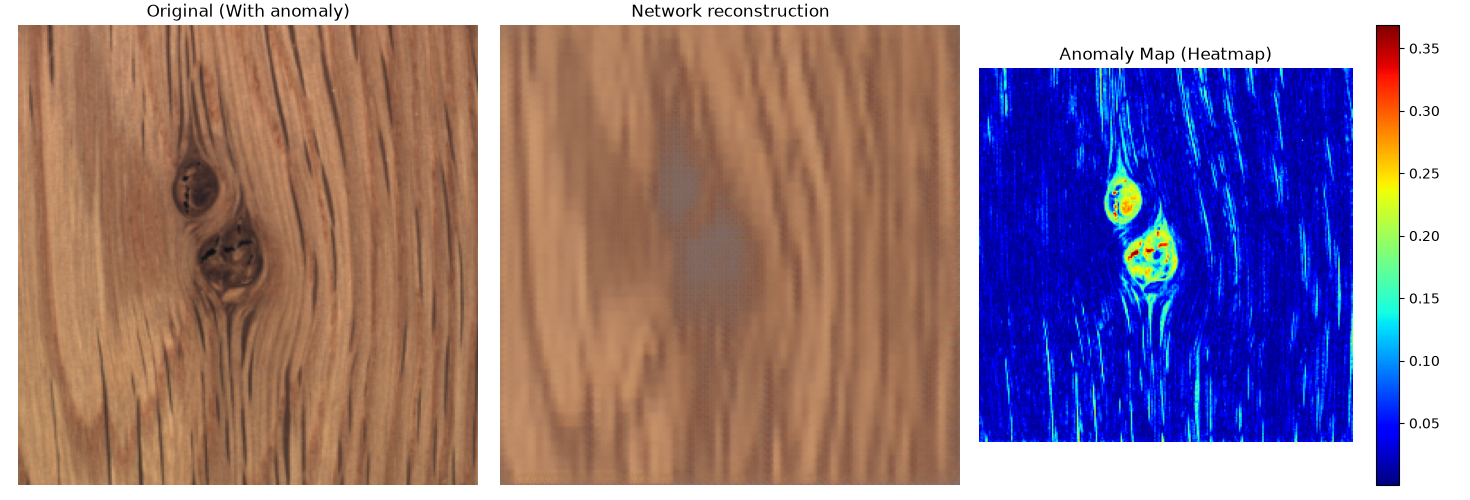
\includegraphics[width=\textwidth]{Heatmap_Wood.png}
        \caption{Wood (In-Domain)}
    \end{subfigure}
    
    \vspace{0.4cm} % Dodaje estetyczny odstęp pionowy między obrazkami
    
    \begin{subfigure}[b]{\columnwidth}
        \centering
        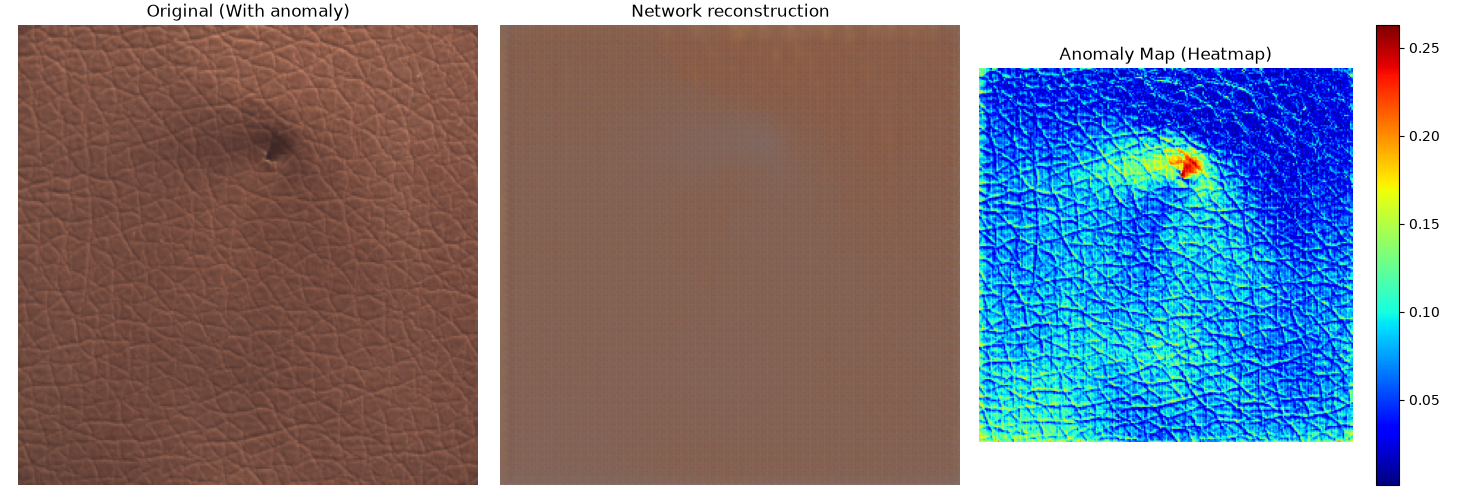
\includegraphics[width=\textwidth]{Heatmap_Leather.png}
        \caption{Leather (Cross-Domain)}
    \end{subfigure}
    
    \vspace{0.4cm}
    
    \begin{subfigure}[b]{\columnwidth}
        \centering
        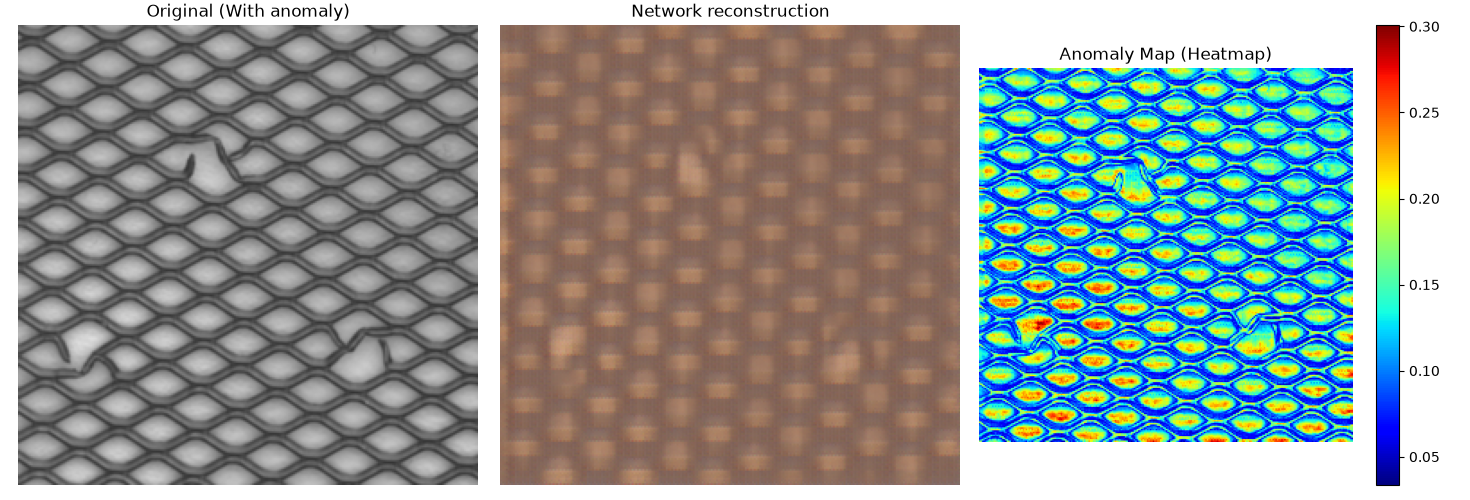
\includegraphics[width=\textwidth]{Heatmap_Grid.png}
        \caption{Grid (Cross-Domain)}
    \end{subfigure}
    
    \caption{Qualitative comparison of generated anomaly heatmaps. The model, trained exclusively on nominal wood, cleanly isolates structural defects in the wood domain (a), but generates massive, global reconstruction errors when exposed to unfamiliar textures like leather (b) and grid (c).}
    \label{fig:heatmaps}
\end{figure}


	
	\subsection{Critical Discussion}

The experimental results yield profound insights into the behavior of the Convolutional Autoencoder under unsupervised anomaly detection constraints. The grid search successfully identified an optimal operating point for the in-domain Wood dataset, confirming that the CAE effectively learned the nominal wood manifold and can reliably project high reconstruction errors over true structural defects.

However, the cross-domain evaluation exposes the strict functional boundaries of this unsupervised framework. At first glance, the cross-domain Recall metric of 100.00\% for both Leather and Grid appears flawless. Yet, a deeper analysis of the confusion matrices reveals a complete operational failure: the model generated exactly zero True Negatives for both unseen datasets. It predicted every single sample—both healthy and anomalous—as defective. Consequently, the Accuracy and Precision metrics merely reflect the dataset's base rate of anomalous samples.

This behavior is entirely consistent with the mathematical foundation of autoencoders. Because the network was forced through a severe dimensional bottleneck using solely wood textures, it physically cannot reconstruct unfamiliar baseline features, such as the repeating weave of a grid or the porous grain of leather. The "healthy" baseline of these new materials yields a massive, global reconstruction error that effortlessly triggers the $\tau_{pixel}$ threshold. As illustrated in Figure \ref{fig:heatmaps}, the residual maps for out-of-domain materials light up completely, effectively blinding the spatial area thresholding mechanism ($\tau_{area}$) to any localized defects.

These findings validate the hypothesis presented in Section 4.1: while unsupervised autoencoders elegantly eliminate the need for costly defect annotations, they are exceptionally domain-sensitive. The model does not learn a universal definition of "anomaly," but rather a strict definition of "non-wood." For industrial application streams, this limitation dictates that a dedicated model must be trained for each distinct material class, or future iterations must integrate domain adaptation techniques to broaden the acceptable boundaries of the healthy feature manifold.





\subsubsection{Theoretical Limitations of the Objective Function}


While the experimental results validate the efficacy of the dual-thresholding pipeline, a critical theoretical limitation resides in the exclusive reliance on the Mean Squared Error (MSE) loss function. MSE computes discrepancies based on absolute pixel intensity, assuming strict spatial independence. Consequently, it is highly sensitive to harmless global illumination shifts or slight structural misalignments, which can inadvertently trigger the $\tau_{pixel}$ threshold and increase false positive rates on complex, non-stationary textures.

To theoretically mitigate this sensitivity, a preprocessing stage could be introduced by transforming the inputs into the HSV color space and applying Contrast Limited Adaptive Histogram Equalization (CLAHE) specifically to the V (Value) channel. This operation would equalize contrast within local tiles while preventing noise amplification, establishing illumination invariance prior to network inference. However, this preprocessing step was deliberately omitted from the current experimental pipeline. The MVTec AD dataset features highly controlled, consistent illumination conditions and lacks background clutter. Applying aggressive contrast equalization to these already pristine images would provide negligible performance benefits and risks destroying subtle, color-based defect signals, thereby negatively impacting the model's high Recall rate. Consequently, relying on standard RGB tensors remains the most resource-efficient strategy for this specific benchmark. While preprocessing techniques such as HSV color space conversion and Contrast Limited Adaptive Histogram Equalization (CLAHE) could potentially enhance feature distinctiveness, they were intentionally omitted to minimize computational overhead and ensure low-latency performance required for real-time inference.

Regarding architectural improvements, recent literature highlights alternative paradigms to mitigate reconstruction blurriness and spatial rigidity. As previously discussed in Section 2.2, integrating structural similarity metrics like CW-SSIM or frequency-aware objective functions such as D3R-Net's FFT penalty could drastically reduce the network's domain sensitivity. While implementing these multi-domain regularizations exceeds the baseline computational scope of this project, they define the optimal trajectory for future work. Such adaptations would allow the network to evaluate complex materials without producing the global reconstruction failures currently observed during cross-domain testing.
	
\section{Conclusion}
	
This project addressed the critical challenge of unsupervised anomaly detection in industrial manufacturing environments, where collecting balanced datasets of defective samples is often impractical. By leveraging the MVTec AD dataset as a foundational benchmark, an anomaly detection pipeline was developed centering on a deep convolutional autoencoder architecture. The model was trained exclusively on defect-free images to learn the manifold of normal textures and objects, allowing anomalies to be isolated through reconstruction error mapping and the subsequent generation of localized anomaly heatmaps.

The experimental evaluation, driven by a systematic hyperparameter grid search, demonstrated the effectiveness of this approach. The optimized pipeline successfully localized defects, achieving a highly prioritized Recall of $98.33\%$, an Accuracy of $92.41\%$, and a strong F1-score of $95.16\%$. The empirical results confirm that the model displays an excellent balance between sensitivity and reliability, optimizing the detection of critical defects while ignoring natural surface fluctuations.

The author’s primary personal contributions to this work encompass the end-to-end design and implementation of the Convolutional Autoencoder architecture, as well as the formulation of the custom dual-thresholding pipeline for anomaly detection. Furthermore, the author independently executed the model training phase, conducted hyperparameter optimization via grid search, and designed the rigorous cross-domain evaluation methodology to empirically test the model's generalization limits.

Despite these promising results, evaluating structural differences across varying datasets underscores a clear limitation: a lightweight convolutional autoencoder optimized for specific industrial patterns cannot instantly adapt to massive topological domain shifts without a modern fine-tuning pipeline. 

To address this and further advance the system, future developments should focus on several key areas. First, the evaluation methodology could be expanded by extracting continuous anomaly scores from the residual maps prior to binary thresholding; this would allow the framework to be assessed using threshold-independent metrics such as the Area Under the Receiver Operating Characteristic (AUROC). Second, the algorithm could transition from empirically defined static thresholds to dynamic statistical modeling; by applying the Three-Sigma rule ($T = \mu + 3\sigma$) to the healthy baseline's mean reconstruction error, the system could establish a self-calibrating threshold. Finally, an exceptionally promising direction lies in transferring this architecture to medical imaging, where it could act as an autonomous clinical screening layer to highlight structural anomalies in X-rays or MRI scans without the need for exhaustive pathological annotations.

\section*{Acknowledgments}
	
The author would like to acknowledge the creators of the MVTec AD dataset, which served as the foundational benchmark for training and evaluating the unsupervised anomaly detection models in this project. Recognition is also extended to the researchers whose referenced methodologies guided the architectural and post-processing decisions within this work. 


Additionally, the author acknowledges the use of Google’s Gemini AI, which provided assistance in conducting the literature search for the referenced works, academic proofreading, and generating hardware-specific boilerplate code — the dynamic device allocation logic (cuda/mps/cpu) used to optimize PyTorch execution across different environments.
	
\begin{thebibliography}{9}

    \bibitem{bergmann2019mvtec}
    P. Bergmann, M. Fauser, D. Sattlegger, and C. Steger,
    ``MVTec AD - A Comprehensive Real-World Dataset for Unsupervised Anomaly Detection,''
    in \textit{Proceedings of the IEEE/CVF Conference on Computer Vision and Pattern Recognition (CVPR)},
    2019.
    
    \bibitem{bionda2022deep}
    A. Bionda, L. Frittoli, and G. Boracchi,
    ``Deep Autoencoders for Anomaly Detection in Textured Images using CW-SSIM,''
    in \textit{Image Analysis and Processing. ICIAP 2022 Workshops}, Springer, pp. 669--680, 2022. doi: 10.1007/978-3-031-06430-2\_56.
    
    \bibitem{filatov2026d3rnet}
    D. Filatov, V. Fedorov, V. Filatova, and A. Zelenchuk,
    ``D3R-Net: Dual-Domain Denoising Reconstruction Network for Robust Industrial Anomaly Detection,''
    \textit{arXiv preprint arXiv:2602.00126}, 2026.

    \bibitem{amini2025mit}
A. Amini and A. Soleimany,
``MIT 6.S191: Introduction to Deep Learning,''
\textit{Massachusetts Institute of Technology}, 2024. [Online]. Available: http://introtodeeplearning.com/

    \bibitem{zhang2021dive}
A. Zhang, Z. C. Lipton, M. Li, and A. J. Smola,
``Dive into Deep Learning,''
\textit{arXiv preprint arXiv:2106.11342}, 2021. [Online]. Available: https://d2l.ai/




        
		%\bibitem{lecun2015deep}
		%Y. LeCun, Y. Bengio, and G. Hinton,
		%``Deep learning,''
		%\textit{Nature}, vol. 521, no. 7553, pp. 436--444, 2015.
		
		%\bibitem{he2016resnet}
		%K. He, X. Zhang, S. Ren, and J. Sun,
		%``Deep residual learning for image %recognition,''
		%in \textit{Proceedings of the IEEE Conference on Computer Vision and Pattern Recognition},
		%pp. 770--778, 2016.
		
		%\bibitem{vaswani2017attention}
		%A. Vaswani, N. Shazeer, N. Parmar, J. Uszkoreit, L. Jones, A. N. Gomez, L. Kaiser, and I. Polosukhin,
		%``Attention is all you need,''
		%in \textit{Advances in Neural Information %Processing Systems},
		%2017.
		
		%\bibitem{lin2014coco}
		%T.-Y. Lin, M. Maire, S. Belongie, J. Hays, P. Perona, D. Ramanan, P. Dollar, and C. L. Zitnick,
		%``Microsoft COCO: Common objects in context,''
		%in \textit{European Conference on Computer Vision},
		%pp. 740--755, 2014.
		
	\end{thebibliography}
	
\end{document}